Neutrinos were introduced into the \emph{Standard Model} as massless particles. But strong evidence from neutrino oscillation experiments indicates that at least one of the neutrino flavors has mass. Neutrino mass terms can be introduced into the \emph{Standard Model} within the Dirac or the Majorana formalism. If the latter describes nature, neutrinos are their own antiparticles. Constrains on the neutrino mass scale come from different aspects of physics. Cosmology constrains the sum of masses of all flavors. Single beta decay experiments measure the mass of the electron neutrino and are sensitive to the neutrino mixing parameters. Neutrinoless double beta decay can only occur if neutrinos are of Majorana type. The decay rate would allow the determination of the effective Majorana neutrino mass.

\section{Neutrinos in \emph{Standard Model}}
\label{sec:sm}
In the \emph{Standard Model} neutrinos are assumed to be fermions with spin 1/2 and rest mass $m_\nu=0$. They always have fixed helicity because there is no frame of reference moving faster than a neutrino, in which the helicity of the neutrino could change its sign. Neutrinos and anti-neutrinos are assumed to be different particles. Lepton numbers +1 and -1 are assigned to them, respectively, and lepton number is conserved. Only left-handed neutrinos and right-handed anti-neutrinos participate in the weak interaction. The field operators of right-handed neutrinos and left-handed anti-neutrinos do not exist in the Lagrangian density of weak interaction.

New experimental evidence, particularly neutrino oscillations, made a modification and extension of the \emph{Standard Model} necessary. Crucial theoretical considerations and experimental observations are briefly reviewed in the following.

The neutrino was postulated to exist by W. Pauli in 1930~\cite{Pau30} in order to explain the continuous energy spectrum of electrons emitted from beta decay without abandoning the law of energy conservation. He assumed that it was a neutral fermion with spin 1/2, and its mass was of the same order of magnitude as the electron mass. E.  Fermi soon developed his theory of beta decay~\cite{Fer33,Fer34}. He investigated the influence of the neutrino mass on the shape of beta spectrum and inferred that $m_\nu \approx 0$ by comparing the calculation to the experimental data. A precise measurement of the beta spectrum of tritium by L. Langer and R. Moffat in 1952~\cite{Lan52} gave an upper limit on the rest mass of the neutrino, $m_\nu < 250 \mbox{eV} = 0.002m_e$. The neutrino was assumed to be massless afterwards. Although the upper limit was pushed down again and again by later experiments, the possibility that neutrinos have very small masses was never completely ruled out, and was strongly supported by the neutrino oscillation experiments.

Beta plus decay was observed by I. Curie and J. F. Joliot in 1934~\cite{Cur34}. Beta decay and beta plus decay in a nucleus can be noted as follows:
\begin{equation}
  \label{eq:bd}
  \beta\mbox{-decay: } n \rightarrow p+e^{-}+\bar{\nu}_e ,
\end{equation}
\begin{equation}
  \label{eq:bpd}
  \beta^+\mbox{-decay: } p \rightarrow n+e^{+}+\nu_e .
\end{equation}
According to Fermi's theory, the following processes also have to exist:
\begin{equation}
  \label{eq:enab}
  e^{+} + n \rightarrow p + \bar{\nu}_e ,
\end{equation}
\begin{equation}
  \label{eq:epab}
  e^{-} + p \rightarrow n + \nu_e ,
\end{equation}
where instead of $e^{-/+}$ emission $e^{+/-}$ are absorbed. Process~\ref{eq:epab} occurring in a nucleus is called electron capture (EC in short). It was observed by L. W. Alvarez in 1938~\cite{Alv38}. The inverse process of \ref{eq:enab} was used by F. Reines and C. L. Cowan, Jr., to detect neutrinos from a nuclear reactor~\cite{Cow56, Rei56}. They proved for the first time that neutrinos do exist in nature.

Whether neutrinos accompanying $e^{+}$ and $e^{-}$ are identical was of great interest at that time. Consider the inverse process of EC,
\begin{equation}
  \label{eq:nunab}
  \nu_e + n \rightarrow p + e^{-} ,
\end{equation}
which, theoretically speaking, also have to exist~\footnote{The process was experimentally proved to exist and used to detect solar neutrinos in many experiments.}. If $\bar{\nu}$ and $\nu$ were identical, the following reaction, where $\nu_e$ is replaced by $\bar{\nu}$, could happen:
\begin{equation}
  \label{eq:bnun}
  \bar{\nu}_e + n \rightarrow p + e^{-}.
\end{equation}
This was investigated by R. Davis in 1955~\cite{Dav55,Dav56}. He was looking for
\begin{equation}
  \label{eq:bnucl}
  \bar{\nu}_e + \, ^{37} \! \text{Cl} \rightarrow \, ^{37} \! \text{Ar} + e^{-}
\end{equation}
and reported a negative result. Before the observation of parity violation and neutrino oscillations this result supported the idea that $\bar{\nu}$ and $\nu$ are intrinsically different particles. To formulate this idea theoretically different \emph{lepton numbers} were assigned to $e^{-}, e^{+}, \nu_e$ and $\bar{\nu}_e$:
\begin{equation}
  \label{eq:ln}
  +1 \mbox{ for }e^{-}, \nu_e, \mbox{   }-1 \mbox{ for
}e^{+},\bar{\nu}_e,
\end{equation}
and required to be conserved in the interaction. The reaction described by eq. \ref{eq:bnucl} is thus forbidden by lepton number conservation.

In 1956 T. D. Lee and C. N. Yang found the existing evidence for parity conservation in weak interaction unsatisfactory and specified the experiments required~\cite{Lee56}. Soon after parity violation was observed in the beta decay of $^{60}$Co~\cite{Wu57} and the creation and decay of muons~\cite{Gar57,Fri57}. Lee and Yang~\cite{Lee57} and some other authors~\cite{Sal57,Lan57} started to apply the so-called two-component model~\cite{Wey29} to the weak interaction. According to this model only the left-handed neutrino and right-handed anti-neutrino or right-handed neutrino and left-handed anti-neutrino participate in the weak interaction. In 1958 an elegant experiment was carried out by M. Goldhaber \textit{et al.} to see whether the right-handed or left-handed components were preferred by nature~\cite{Gol58}. By measuring the polarization of $\gamma$-rays emitted from $^{152}$Sm* created in the electron capture, $^{152}$Eu$(e^-,\nu)$, they inferred that neutrinos from $^{152}$Eu$(e^-,\nu)$ were left-handed. Now the absence of reaction \ref{eq:bnucl} could be explained in two different ways:
\begin{itemize}
\item $\bar{\nu}$ and $\nu$ behave differently because they are   intrinsically different particles.
\item $\bar{\nu}$ and $\nu$ behave differently only because they have   different helicities.
\end{itemize}

In summary, though the \emph{Standard Model} of weak interaction is a very successful theory some modifications were still possible:
\begin{itemize}
\item neutrinos could be massive;
\item $\bar{\nu}$ and $\nu$ might not be different, and hence lepton   number is not conserved.
\end{itemize}


\section{Neutrino oscillations}
\label{sec:osci}
The assumption that neutrinos were massless was challenged in 1969 by Gribov and Pontecorvo who predicted that neutrinos might oscillated into different flavors if some of them were massive and if there was mixing between them~\cite{Gri69}. This is what is called \emph{neutrino oscillations}.

The theory of \emph{neutrino oscillations} can be briefly summarized as follows: the mass eigenstates of neutrinos, $\nu_{i}$, are not the same as their weak interaction eigenstates, $\nu_{\alpha}$; the latter is a combination of the former
\begin{equation}
  \label{eq:osci}
  |\nu_{\alpha}\rangle=\sum_{i}U^{*}_{\alpha i}|\nu_{i}\rangle,
\end{equation}
where $\alpha=e,\mu,\tau$, and $i=1,2,3$, and $U$ is a unitary matrix referred to as the Pontecorvo-Maki-Nakagawa-Sakata(PMNS) matrix. A common parameterization of the PMNS matrix is
\begin{equation}
  \label{eq:pmns}
  \begin{array}{rcl}
    U = \left(\begin{array}{ccc}
        1 & 0 & 0 \\ 0 & \cos\theta_{23} & \sin\theta_{23} \\ 0 &         -\sin\theta_{23} & \cos\theta_{23}
      \end{array}\right) &\times&
    \left(\begin{array}{ccc}
        \cos\theta_{13} & 0 & \sin\theta_{13}e^{-i\delta} \\ 
        0 & 1 & 0 \\ -\sin\theta_{13}e^{i\delta} & 0 & \cos\theta_{13}
      \end{array}\right) \\\times
    \left(\begin{array}{ccc}
        \cos\theta_{12} & \sin\theta_{12} & 0 \\ -\sin\theta_{12} &         \cos\theta_{12} & 0 \\ 0 & 0 & 1
      \end{array}\right) &\times&
    \left(\begin{array}{ccc}
        e^{i\alpha_1/2} & 0 & 0 \\ 0 & e^{i\alpha_2/2} & 0 \\ 0 & 0 & 1
      \end{array}\right),
  \end{array}
\end{equation}
where $\theta_{ij}$'s are three mixing angles, $\delta$, $\alpha_1$ and $\alpha_2$ are CP-violating phases. Especially, $\alpha_1$ and $\alpha_2$ also known as Majorana phases, have physical consequences only, if neutrinos are Majorana particles. The probability that a neutrino originally of flavor $\alpha$ will be observed as having flavor $\beta$ after traveling a distance $L$ is
\begin{equation}
  \label{eq:pa2b}
  \begin{array}{ccccl}
    P_{\alpha \rightarrow \beta} &=& \left| \left\langle                 \nu_{\beta}|\nu_{\alpha}(t) \right\rangle \right|^{2} &=&     {\displaystyle \left|       \sum_{i}U_{\alpha i}^{*}U_{\beta i}e^{-i           m_{i}^2 L/2E} \right|^{2}}\\ &=& \delta_{\alpha\beta} &-&     4{\displaystyle \sum_{i>j}Re(U_{\alpha         i}^{*}U_{\beta         i}U_{\alpha j}U_{\beta j}^{*})\sin^{2}(\Delta     m_{ij}^{2}       \frac{L}{4E})}\\ & & &+& {\displaystyle 2\sum_{i>j}Im(U_{\alpha         i}^{*}U_{\beta i}U_{\alpha j}U_{\beta j}^{*})\sin(\Delta       m_{ij}^{2}\frac{L}{2E})},
  \end{array}
\end{equation}
where $\Delta m^{2}_{ij}$ is the squared mass difference between the
two mass eigenstates $m^{2}_{i} - m^{2}_{j}$ and $E$ is the
average energy of the mass eigenstates.

Oscillations would not occur ($P_{\alpha \rightarrow \beta} = 0$) if neutrinos are all massless or all masses are degenerate ($\Delta m^{2} = 0$) or there is no mixing ($\theta = 0$); \textit{i.e.} if there are neutrino oscillations at least one neutrino must have mass and it must mix.

\subsection{Solar neutrinos}
\label{sec:solar}
The hypothesis of neutrino oscillations was first used to explain the problem of the solar neutrino flux~\cite{Dav64,Dav68}, which was measured to be lower than that was predicted by the standard solar model~\cite{Bah98}. This explanation was at first not widely accepted because it required very large neutrino mixing and a fine-tuned squared mass difference to fit the distance between the Sun and the Earth. The uncertainties of the standard solar model were used to resolve the problem instead, \textit{i.e.} to deny its existence.

It was first realized by L. Wolfenstein in 1978 that neutrinos propagating in matter have different effective masses than those in vacuum due to charged current coherent forward scattering of electron neutrinos with electrons in matter~\cite{Wol78}. Since neutrino oscillations depend upon the squared mass difference of the neutrinos, they can be different in matter than in vacuum. S. P. Mikheyev and A. Yu. Smirnov noticed in 1986 that, even if the intrinsic oscillations were small, the matter effect could still cause maximal mixing between electron neutrinos and the other flavors~\cite{Mik86}. Their observation is called MSW effect. Since this mechanism did not require the intrinsic mixing angle to be very large and the squared mass difference fine-tuned to fit the distance between the sun and the earth, people started to believe that neutrino oscillations might be the answer to the solar neutrino flux problem.

The experiments~\cite{Hir89,Aba91,Ans92} following the chlorine experiment all observed solar neutrino deficits which were explained as the result of neutrino oscillations. The ranges of allowed neutrino mixing parameters were narrowed step by step. However, the most convincing evidence came from the combined results from the Sudbury Neutrino Observatory (SNO) and Super-Kamiokande in 2001~\cite{Ahm01,Fuk01}. SNO measured precisely the neutrino flux through the charged current (CC) reaction, $\phi^{CC}(\nu_e)$, which is sensitive exclusively to $\nu_e$. Super-Kamiokande measured precisely the neutrino flux through the elastic scattering (ES), $\phi^{ES}(\nu_\alpha)$, which is sensitive to all active neutrino flavors ($\alpha = e, \mu, \tau$). If $\nu_e$s from the sun change into other flavors $\phi^{CC}(\nu_e)$ should be smaller than $\phi^{ES}(\nu_\alpha)$. The experimental result was that $\phi^{CC}(\nu_e)$ was smaller than $\phi^{ES}(\nu_\alpha)$ with a $3.3\sigma$ difference. Since the result did not rely on solar model flux calculations the solar neutrino oscillation was finally well established.

low energy solar neutrino experiments...

\subsection{Atmosphere neutrinos}
\label{sec:atmo}
Studies of atmospheric neutrinos also indicated the existence of neutrino oscillations. In the early 1980s several massive detectors were built to search for proton decays. Neutrinos created by cosmic rays in the atmosphere were studied in detail as a source of background events. A deficit in the muon neutrino flux relative to the electron neutrino flux compared with the calculation was found in two experiments, IMB~\cite{Hai86} (1986) and Kamiokande~\cite{Hir88} (1988). The IMB group, however, took the conservative attitude and ascribed the deficit to some unknown systematics. On the other hand, the Kamiokande group, relying on its capability to clearly separate $e$ and $\mu$ events, interpreted it as evidence for neutrino oscillations.

Kamiokande further investigated this phenomenon and found in 1994 that the flux of high energy muon neutrinos showed a nontrivial zenith-angle dependence that could best be explained by $\nu_\mu$ oscillating to $\nu_\tau$~\cite{Fuk94}. This still did not convince everybody because the oscillation interpretation required very large mixing between two neutrinos which was not considered reasonable. Finally, Super-Kamiokande, the enlarged facility of Kamiokande, showed that all aspects of atmospheric neutrino data were consistent with neutrino oscillation between $\nu_\mu$ and $\nu_\tau$, and the mixing was nearly maximal (1998)~\cite{Fuk98}.

\subsection{Reactor neutrinos}
\label{sec:reactor}
Compared to solar and atmospheric neutrinos the neutrinos from artificial sources, reactors and accelerators, allow precise measurements of the oscillation parameters under more controlled and better understood conditions. Reactor neutrino experiments detect anti-neutrinos from the decays of radioactive fission products in the nuclear fuel. The detector can be constructed at varying distances from the source, and hence variable sensitivity to different oscillation parameters. For instance, KamLAND~\cite{Kam03} has a flux weighted average distance of $\sim180$ km from more than 60 nuclear reactors around. It has better precision in the measurement of the mass difference $\Delta m^{2}_{21}$ but is less sensitive to the mixing angle $\theta_{12}$ than the solar neutrino experiments. The combined fit of its and the solar neutrino experiments data gives the best results on $\Delta m^{2}_{21}$ and $\sin^{2}\theta_{12}$~\cite{Kam08}. KamLAND can also detect the anti-neutrino energy. The energy spectrum clearly reflects the oscillation pattern, thus excludes hypothesis such as neutrino decay and decoherence.

The Chooz experiment, instead, was situated only $\sim1000$ m away from the reactors. It was sensitive to the PMNS matrix element $U_{e3}^{2}$, and gave the best limit on $\sin^{2}\theta_{13}$~\cite{Cho03}. Since $\theta_{13}$ modulates the effect of CP violation, more precise measurement of $\theta_{13}$ is of great interest. Using an extra detector near the reactors the systematic uncertainties related to neutrino production and interaction cancel in relative measurements~\cite{Koz03}. Following this idea, three experiments, Double Chooz~\cite{Dbc06}, Daya bay~\cite{Day07} and RENO~\cite{Ren08}, are under construction. Daya Bay aims at $\sin^{2}2\theta_{13}$ sensitivity better than 0.01 while Double Chooz and RENO aim at $0.02 \sim 0.03$ at $90\%$ C.L. for 3 years measuring time.

\subsection{Accelerator  neutrinos}
\label{sec:acce}
Neutrino beams from accelerators usually contain dominantly muon neutrinos or anti-neutrinos. Their energy is adjested to the application and ranges from almost 0 to several hundred GeV. The close-far detector configuration is also used in some cases. The accelerator neutrino experiments hence can investigate different oscillation phenomena. K2K~\cite{K2K06} and MINOS~\cite{Min06} measure the muon neutrino deficit and energy distribution in the far detector normalized to the observations in the close one. The aim is to precisely measure the squared mass difference and the mixing angle. Opera~\cite{Ope06} searches for the appearance of $\tau$ neutrinos in the CERN muon neutrino beam. KARMEN~\cite{Kar03} and LSND~\cite{Dod06} searched for the appearance of electron neutrinos in their muon neutrino beams. The former reported negative result, while the latter claimed the existence of $\nu_{\mu}/\bar{\nu}_{\mu} \rightarrow \nu_{e}/\bar{\nu}_{e}$ oscillations, but with quite a different mass difference squared as found in solar and atmosphere oscillation experiments. This could only be accommodated by the existence of extra sterile neutrinos. The evidence provided by LSND was partially refuted recently by MiniBOONE~\cite{Agu07}. Further scrutiny is needed to exclude some more exotic possibilities. Two future experiments, T2K~\cite{T2K05} and NOvA~\cite{Nov05}, are under construction to search for electron neutrino appearance, to measure the mixing angle $\theta_{13}$ and the CP violation phase $\delta$.

\subsection{Summary of neutrino oscillations}
\label{sec:allo}
Neutrino oscillations have been observed not only in solar and atmosphere neutrino experiments but also in reactor and accelerator neutrino experiments. It is established that neutrinos do have masses. Comprehensive data analyses of the mass differences squared and the mixing parameters based on the 3-neutrino mixing scheme can be found in the latest \emph{Review of Particle Physics}~\cite{PDG08}. Since the oscillation experiments can only measure the mass differences between the neutrino mass eigenstates and cannot determine the signs of $\Delta m^{2}_{23}$, there are two interesting questions left as shown in Fig~\ref{fig:hie}:
\begin{itemize}
\item what are the absolute values of the neutrino masses?
\item what is the real mass hierarchy? Does it correspond to the   (normal) mass hierarchy of the charged lepton sector or is it   inverted?
\end{itemize}
\begin{figure}[tbhp]
  \centering
  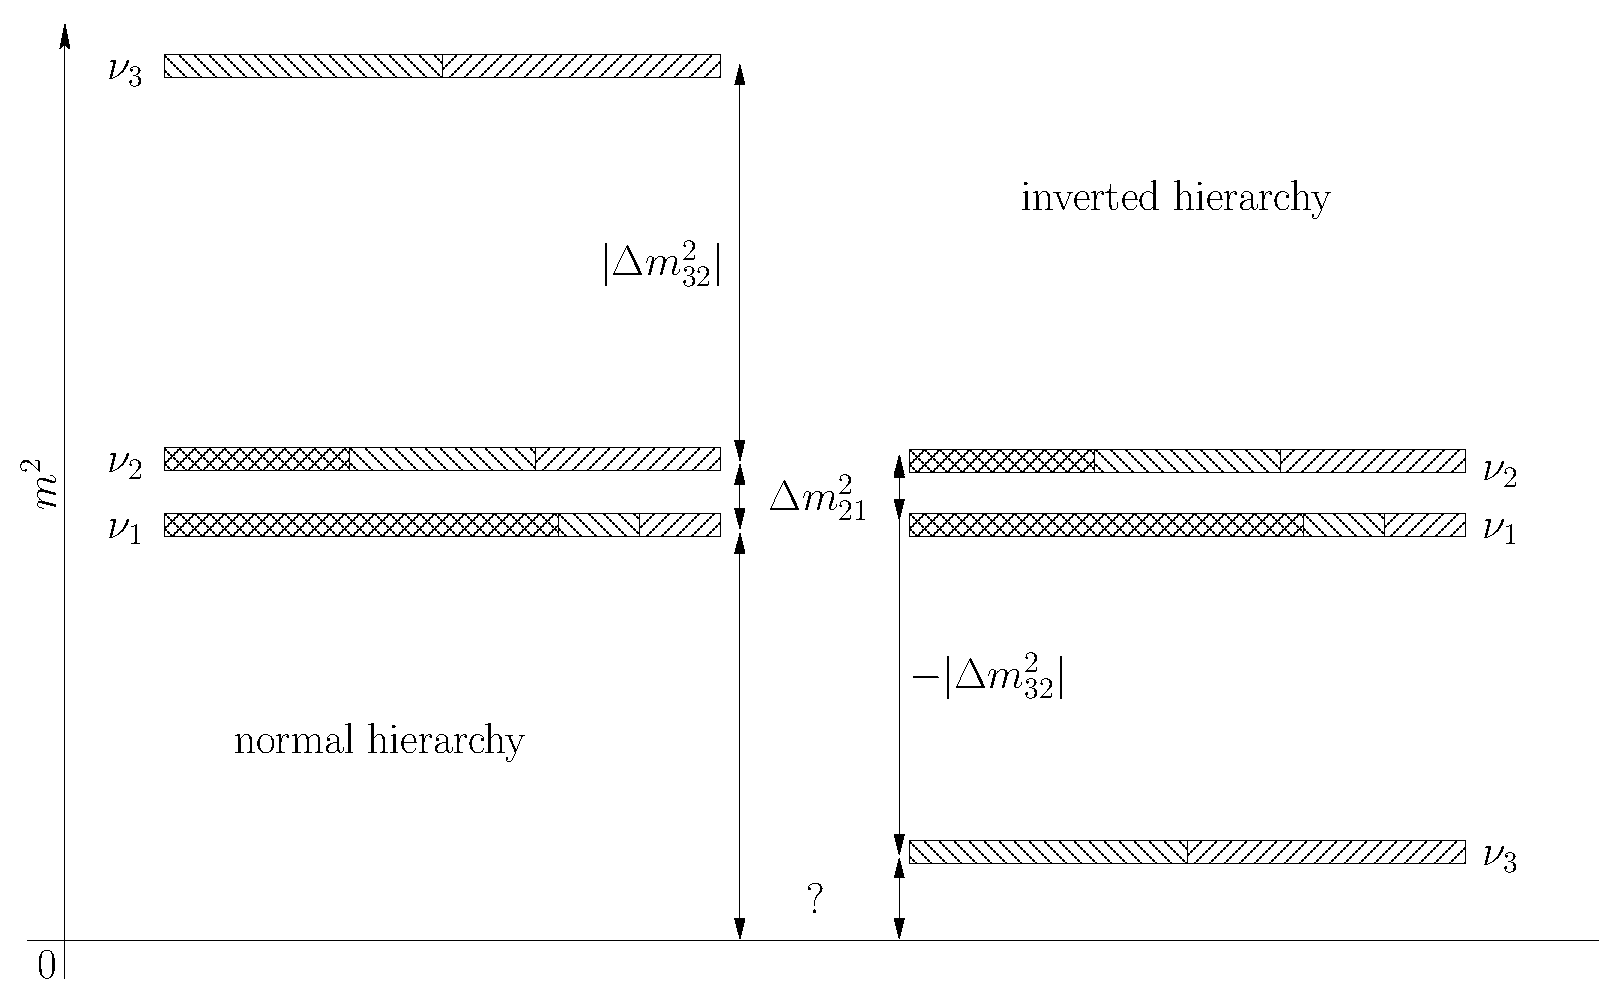
\includegraphics[width=0.8\textwidth]{massHierarchy.eps}  
  \caption{Possible neutrino mass squared spectra. Oscillation     experiments can neither help to determine the absolute mass scale     nor to distinguish between normal and inverted hierarchy.}
  \label{fig:hie}
\end{figure}


\section{Neutrino mass terms}
\label{sec:nema}
The observation of neutrino oscillations makes the introduction of
neutrino mass terms into the \emph{Standard Model} necessary.
\subsection{Dirac mass term}
\label{sec:dirac}
The most straightforward approach to introduce the mass term is to follow the same procedure as for the electron, \textit{i.e.} the lepton obtains mass by coupling to the Higgs field. The mass term of the electron can be expressed as
\begin{equation}
  \label{eq:dme}
  -\mathcal{L}_{e} \equiv m_{e}\bar{e}e = g_{e}\langle      
  h^{0}\rangle \bar{e}e,
\end{equation}
with $m_{e} = g_{e} \langle h^{0}\rangle$, where $g_e$ is the coupling strength of electron field $e$ to Higgs field, and $\langle h^{0} \rangle$ is the vacuum expectation value for the Higgs field. Similarly, the Dirac mass term of the neutrino can be expressed as
\begin{equation}
  \label{eq:dmnu}
  -\mathcal{L}_{\nu}^{D} \equiv m_{D}\bar{\nu}\nu = g_{\nu} \langle       h^{0} \rangle \bar{\nu}\nu,
\end{equation}
with $m_{D} = g_{\nu} \langle h^{0}\rangle$, where $g_\nu$ is the coupling strength of neutrino field $\nu$ to Higgs field. Since neutrinos are much lighter than their leptonic partners, the coupling strength of the neutrino field to the Higgs field has to be much smaller than that of electron:
\begin{equation}
  \label{eq:gg}
  g_{\nu} \ll g_{e}.
\end{equation}
After introducing the Dirac mass term the question arises why
neutrinos couple to the Higgs field so weakly compared to their
leptonic partners. And since an insertion of the Dirac matrix $\gamma^{5}$ yields
\begin{equation}
  \label{eq:2psi}
  \bar{\nu}\nu = \bar{\nu}    
  \left(\frac{1+\gamma^5}{2}+\frac{1-\gamma^5}{2}\right)
  \left(\frac{1+\gamma^5}{2}+\frac{1-\gamma^5}{2}\right) \nu =
  \overline{\nu_{L}}\nu_{R}+\overline{\nu_{R}}\nu_{L},
\end{equation}
a right-handed partner of the left-handed neutrino and a left-handed partner of the right-handed anti-neutrino must be introduced in order to prevent $m_{D}\bar{\nu}\nu$ to vanish.

\subsection{Majorana mass terms}
\label{sec:major}
Theoretically, $\overline{\psi^{c}}\psi^{c}, \bar{\psi}\psi^{c}$ and $\overline{\psi^{c}}\psi$ are also possible mass terms, where $\psi^{c}$ is the charge conjugate of $\psi$. $\overline{\psi^{c}} \psi^{c}$ is equivalent to $\bar{\psi}\psi$. $\bar{\psi}\psi^{c}$ and $\overline{\psi^{c}}\psi$ cannot be mass terms for electrons or quarks because they destroy or create two particles of equal electric charge. However, they can be used as mass terms for neutrinos, because neutrinos do not have electric charge. These mass terms destroy or create two particles of the same lepton number, hence violate lepton number conservation and are called Majorana mass terms:
\begin{equation}
  \label{eq:mmt}
  -\mathcal{L}_{\nu}^{M} \equiv \frac{1}{2}m_{L} \left(
    \overline{\nu_{L}}(\nu_{L})^{c} +                  \overline{(\nu_{L})^{c}}\nu_{L}
  \right) + \frac{1}{2}m_{R} \left(
    \overline{(\nu_{R})^{c}}\nu_{R} +                       \overline{\nu_{R}}(\nu_{R})^{c} \right),
\end{equation}
where $m_{L}$ and $m_{R}$ are two independent constants. 

\subsection{Generic mass terms}
\label{sec:genma}
Nature could reflect a combination of the Dirac and Majorana mass terms:
\begin{equation}
  \label{eq:dmm}
  \begin{array}{ccl}
    -2\mathcal{L}_{\nu}^{D+M} &\equiv& -2\mathcal{L}_{\nu}^{D}             -2\mathcal{L}_{\nu}^{M}\\ &=& \displaystyle{( 
      m_{D}\overline{\nu}\nu +
      m_{D}\overline{\nu^{c}}\nu^{c} )}\\ &+& \displaystyle{(             m_{L}\overline{\nu_{L}}(\nu_{L})^{c} +                         m_{L}\overline{(\nu_{L})^{c}}\nu_{L} +                   m_{R}\overline{(\nu_{R})^{c}}\nu_{R} +                                      m_{R}\overline{\nu_{R}}(\nu_{R})^{c})}\\ &=&\displaystyle{
      m_{D}\overline{\nu_{L}}\nu_{R} +
      m_{D}\overline{(\nu_{R})^{c}}(\nu_{L})^{c} +
      m_{L}\overline{\nu_{L}}(\nu_{L})^{c} + 
      m_{R}\overline{(\nu_{R})^{c}}\nu_{R} + h.c.},
  \end{array}
\end{equation}
where $h.c.$ stands for Hermitian conjugate. Introducing the notation $\nu^{c}_{L,R} \equiv (\nu^{c})_{L,R} = (\nu_{R,L})^{c}$ eq.~\ref{eq:dmm} can be written as
\begin{equation}
  \label{eq:mm}
  -2\mathcal{L}_{\nu}^{D+M} =       \left(\overline{\nu_{L}},\overline{\nu^{c}_{L}}\right)
  \left(\begin{array}{cc}m_L & m_D \\ m_D & m_R\end{array}\right)
  \left(\begin{array}{c}\nu^{c}_R \\ \nu_R\end{array}\right) + h.c.
\end{equation}
By choosing a orthogonal matrix $\mathcal{U}$ ($\mathcal{U}^{T}
\mathcal{U} = 1$) such that
\begin{equation}
  \label{eq:mmat}
  \mathcal{U}^{T}\left(\begin{array}{cc}m_L & m_D \\ m_D &       
m_R\end{array}\right)\mathcal{U} = 
  \left(\begin{array}{cc}\epsilon_{1}m_1 & 0 \\ 0 &            
\epsilon_{2}m_2\end{array}\right),
\end{equation}
where $m_{1}, m_{2} > 0$, $\epsilon_{1,2} = \pm 1$, and defining
\begin{equation}
  \label{eq:mvet}
  (\nu_{1L}, \nu_{2L}) = \left( \overline{\nu}_{L},                 \overline{\nu^{c}_{L}} \right) \mathcal{U},
  \left(\begin{array}{c} \nu^{c}_{1R} \\            
      \nu^{c}_{2R}\end{array}\right) = \mathcal{U}^{T}
  \left(\begin{array}{c} \nu^{c}_{R} \\ \nu_{R} \end{array}\right),
\end{equation}
eq.~\ref{eq:mm} can be rewritten as
\begin{equation}
  \label{eq:m12}
  \mathcal{L}_{\nu}^{D+M} = m_{1}\overline{\nu_{1L}}\nu^{c}_{1R} +  
  m_{1}\overline{\nu^{c}_{1R}}\nu_{1L} +
  m_{2}\overline{\nu_{2L}}\nu^{c}_{2R} +  
  m_{2}\overline{\nu^{c}_{2R}}\nu_{2L}.
\end{equation}
With
\begin{equation}
  \label{eq:mafi}
  \phi_{1} = \nu_{1L} + \epsilon_{1}\nu^{c}_{1R}
  \mbox{\ \ \ and \ \ \ }
  \phi_{2} = \nu_{2L} + \epsilon_{2}\nu^{c}_{2R},
\end{equation}
eq.~\ref{eq:mm} reduces to
\begin{equation}
  \label{eq:mv}
  -2\mathcal{L}_{\nu}^{D+M} = m_{1}\bar{\phi}_{1}\phi_{1} +
  m_{2}\bar{\phi}_{2}\phi_{2}
\end{equation}
Obviously,
\begin{equation}
  \label{eq:mach}
  \phi^{c}_{k} = (\nu_{kL})^{c} + \epsilon_{k}(\nu^{c}_{kR})^{c} =
  \epsilon_{k}\phi_{k}, ~~~ (k=1,2)
\end{equation}
\textit{i.e.} $\phi$ is its own anti-particle, and hence of Majorana type.

If $m_{R} \gg \mathcal{O}(m_{e}), m_{L}=0$ and $m_{D} \approx \mathcal{O}(m_{e})$,
\begin{equation}
  \label{eq:seesaw}
  m_{1} = \frac{m^{2}_{D}}{m_{R}}\ll m_{D}  \mbox{\ \ \ and \ \ \ }  
  m_{2} = m_{R}(1+\frac{m^{2}_{D}}{m^{2}_{R}}) \approx m_{R} \gg m_{D}.
\end{equation}
Thus, if there exists a very heavy Majorana state $\phi_2$, the other state $\phi_1$ would be much lighter than $m_e$. This is the so-called seesaw mechanism.

In summary, both Dirac and Majorana mass terms should be taken into account. For fermions carrying charge or similar quantum numbers Majorana mass terms are forbidden. This is not the case for neutrinos. Majorana neutrinos $\phi_{1}, \phi_{2}$ can be constructed out of combinations of Dirac and Majorana fields. Using the seesaw mechanism the tiny neutrino masses can be explained naturally.

\section{Probing neutrino masses}
\label{sec:pnm}
The current neutrino oscillation experiments cannot address both problems, the absolute mass scale and the mass hierarchy. Three major methods to address the questions are:
\begin{description}
\item[Cosmological observations] which are sensitive to the sum of all neutrino masses $\Sigma$,
\item[Single beta decay experiments] which are sensitive to the   effective electron neutrino mass $m_{\beta}$,
\item[Neutrinoless double beta ($0\nu\beta\beta$) decay experiments] which are sensitive   to the effective Majorana neutrino mass $m_{\beta\beta}$.
\end{description}

\subsection{Cosmological observations}
\label{sec:coob}
According to the standard model of cosmology neutrinos affect the evolution of the universe in three aspects. First, the number of neutrino flavors, $N_{\nu}$, affects the abundances of light elements in the early universe which are reflected in the cosmic microwave background (CMB). Using current CMB data, the value of $N_{\nu}$ is determined to be $1.8 \sim 3.3$~\cite{Oli02}. Secondly, if our universe is flat, the energy density of the universe $\Omega = \Omega_{\Lambda} + \Omega_{cd} + \Omega_{b} + \Omega_{\nu} = 1$, where $\Omega_{\Lambda}, \Omega_{cd}, \Omega_{b}$ and $\Omega_{\nu}$ indicate the contribution to the energy density from dark energy, cold dark matter, baryons and neutrinos, respectively. If neutrinos have substantial mass, the percentages of the other components of the universe change as does the evolution of the universe. This would be reflected in the CMB data. Finally, the large-scale structures (LSS) existing today indicate the existence of small initial density fluctuations. Relativistic neutrinos, as weakly interacting particles, could escape without interaction from areas of high density to areas of low density (free streaming); hence, could wash out the  fluctuations. The larger the neutrino masses, the stronger is the effect. The data on anisotropies in LSS thus gives access to neutrino masses. 

Cosmological observations are only sensitive to the sum of the neutrino masses
\begin{equation}
  \label{eq:msum}
  \Sigma \equiv \sum_{i}m_{i}.
\end{equation}
They are not sensitive to the oscillation parameters and cannot distinguish between Dirac and Majorana neutrinos. However, the limit on the sum of neutrino masses from cosmology does help to answer the questions left by the oscillation experiments. Fig.~\ref{fig:sumVSlightest}, taken from Ref.~\cite{Str05}, shows the expected range of the sum of the neutrino masses as a function of the lightest neutrino mass. The regions noted with $\Delta m^{2}_{32}<0$ and $\Delta m^{2}_{32}>0$ are the allowed regions in case of inverted and normal hierarchy, respectively. If the limit was as low as $\sim 0.08$~eV, the normal and inverted hierarchy could be distinguished. Considering only the CMB data the $2\sigma$ (95\% CL) constrain on the sum of neutrino masses is 1.19 eV. Taking into account LSS the constrain could go down to the sub eV level~\cite{Fog08}. Several calculations show that the Planck satellite, which is going to be launched soon, can set a limit at the $0.07 \sim 0.25$~eV level~\cite{Pla05}.
\begin{figure}[tbhp]
  \centering
  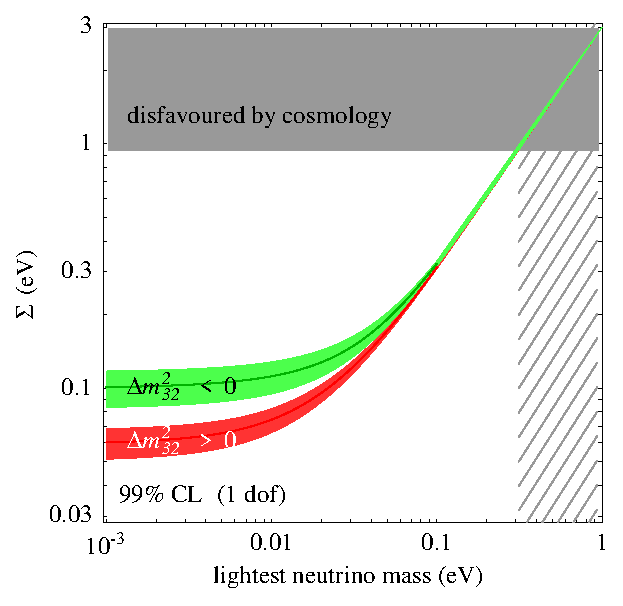
\includegraphics[width=0.5\textwidth]{sumVSlightest.eps}  
  \caption{Expected range of the sum of the neutrino masses $\Sigma$     as a function of the lightest neutrino mass (taken from     Ref.~\cite{Str05}). The regions noted with $\Delta m^{2}_{32}<0$     and $\Delta m^{2}_{32}>0$ are the allowed regions at 99\%     confidence level (CL) in case of inverted and normal hierarchy,     respectively. The darker lines in the middle of the regions     correspond to the central values of the oscillation     parameters. The hatched area is disfavored by the single beta     decay experiments.}
  \label{fig:sumVSlightest}
\end{figure}

Additional information could come from supernova neutrinos.
They would arrive slightly later than $\gamma$-rays from the same
source if they do have mass.

\subsection{Single beta decay}
\label{sec:sbd}
By precisely measuring the shape of the beta decay spectrum around its end point the single beta decay experiments dominantly probe the effective electric neutrino mass
\begin{equation}
  \label{eq:m1b}
  m_{\beta} \equiv \sqrt{\sum_{i=1}m_{i}^{2}|U_{ei}|^{2}}.
\end{equation}
The Dirac or Majorana nature of the neutrino cannot be inferred from $m_{\beta}$ because the phases in the PMNS matrix do not contribute to the absolute values of the $U_{ei}$'s. The MAINZ~\cite{Mai99} and TROITSK~\cite{Tro99} experiments measured $m_{\beta}$ in tritium beta decay. The combined limit is $m_{\beta} < 2.0$ eV at 99\% CL. The sensitivity targeted by the future experiments KATRIN~\cite{Kat01}, also based on tritium decay, and MARE~\cite{Mar05}, based on $^{187}$Re decay, is $\sim 0.2$~eV. Fig.~\ref{fig:m1bVSlightest}, taken from Ref.~\cite{Str05}, shows the expected range of the effective electric neutrino mass $m_{\beta}$ as a function of the lightest neutrino mass. The regions noted with $\Delta m^{2}_{32}<0$ and $\Delta m^{2}_{32}>0$ are the allowed regions in case of inverted and normal hierarchy, respectively. Obviously, the sensitivities of KATRIN and MARE are not good enough to resolve the hierarchy problem.
\begin{figure}[tbhp]
  \centering
  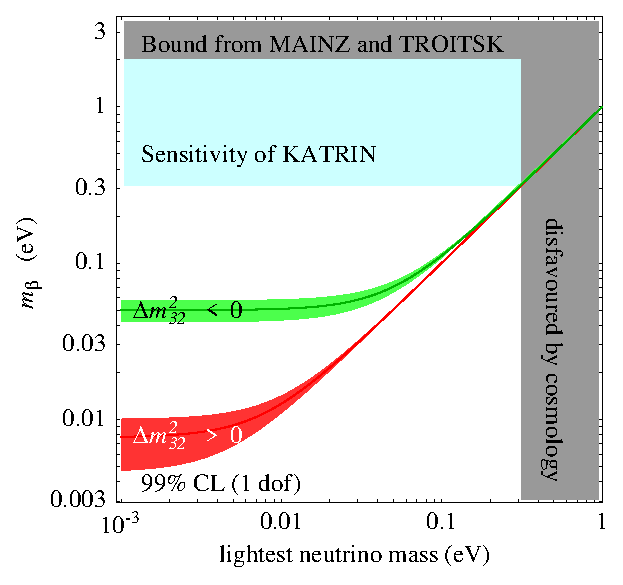
\includegraphics[width=0.5\textwidth]{m1bVSlightest.eps}  
  \caption{Expected range of the effective electron neutrino mass     $m_{\beta}$ as a function of the lightest neutrino mass (taken from     Ref.~\cite{Str05}). The regions noted with $\Delta m^{2}_{32}<0$     and $\Delta m^{2}_{32}>0$ are the allowed regions at 99\%     confidence level (CL) in case of inverted and normal hierarchy,     respectively. The darker lines in the middle of the regions     correspond to the central values of the oscillation parameters. The bounds from cosmology and previous single beta decay experiment are shown with dark background. The sensitivity of KATRIN is shown with lighter background (cyan online).}
  \label{fig:m1bVSlightest}
\end{figure}

\subsection{Neutrinoless double beta decay}
\label{sec:nonubb}
Due to the pairing interaction even-even nuclei are more bound than the odd-odd ones. Take $^{76}_{32}$Ge as an example. It is an even-even nucleus and cannot decay into its nearest neighbor even-odd nucleus $^{76}_{33}$As due to energy conservation. It can, however, decay into the next to nearest neighbor $^{76}_{34}$Se by emitting two electrons (double beta decay) as shown in Fig~\ref{fig:ee2oo}. 
\begin{figure}[tbhp]
  \centering
  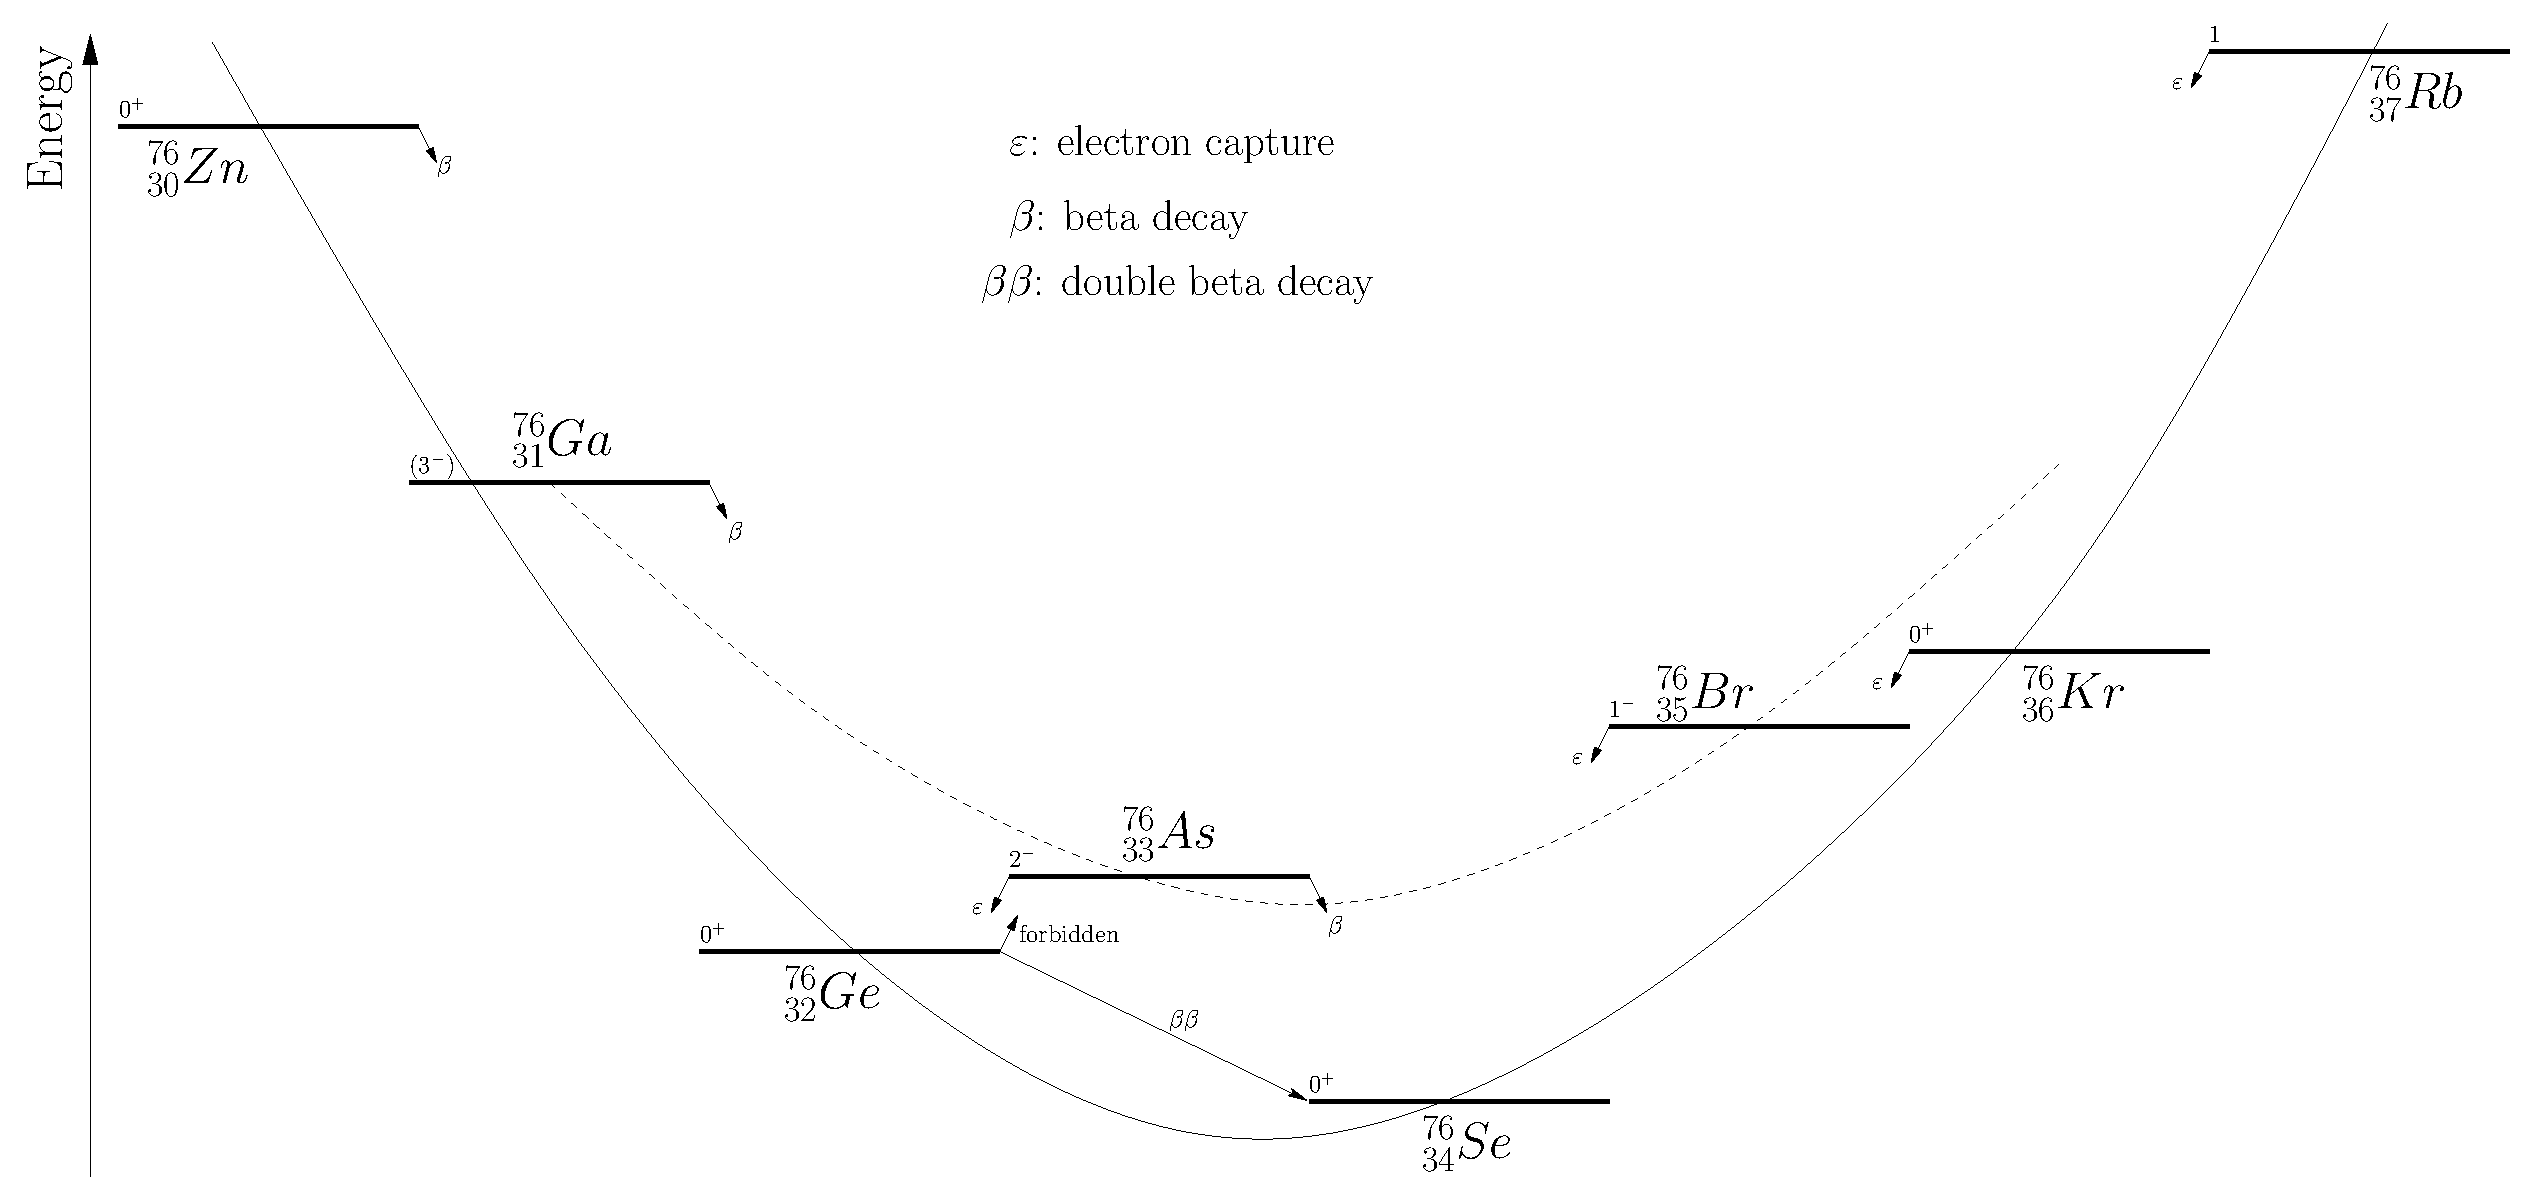
\includegraphics[width=0.9\textwidth]{Espec0nu2b.eps}  
  \caption{Decay sequence of nuclei with $A=76$. Even-even nuclei     (chained with solid parabola) are more bound than the odd-odd     nuclei (chained with dashed parabola). The single beta decay from     $^{76}_{32}$Ge to $^{76}_{33}$As is forbidden due to the energy     conservation.}
  \label{fig:ee2oo}
\end{figure}
If neutrinos are of Dirac type, two neutrinos also have to be emitted in the double beta decay ($2\nu\beta\beta$). If neutrinos have masses and of Majorana type, the neutrino emitted in one beta decay could be absorbed in another and a decay without neutrino emission would become possible. This is the so-called neutrinoless double beta decay ($0\nu\beta\beta$). These two types of double beta decays are denoted:
\begin{eqnarray}
  2\nu\beta\beta: (Z,A) &\rightarrow& (Z+2,A) + 2e^{-} +
  2\bar{\nu}_{e}, \\\label{eq:2nu2b}
  0\nu\beta\beta: (Z,A) &\rightarrow& (Z+2,A) + 2e^{-},
\label{eq:0nu2b}
\end{eqnarray}
where $Z$ is the charge of the nucleus and $A$ is the atomic number.
The Feynman diagrams of both processes are shown in
Fig.~\ref{fig:2bdecay}.
\begin{figure}[tbhp]
  \centering
  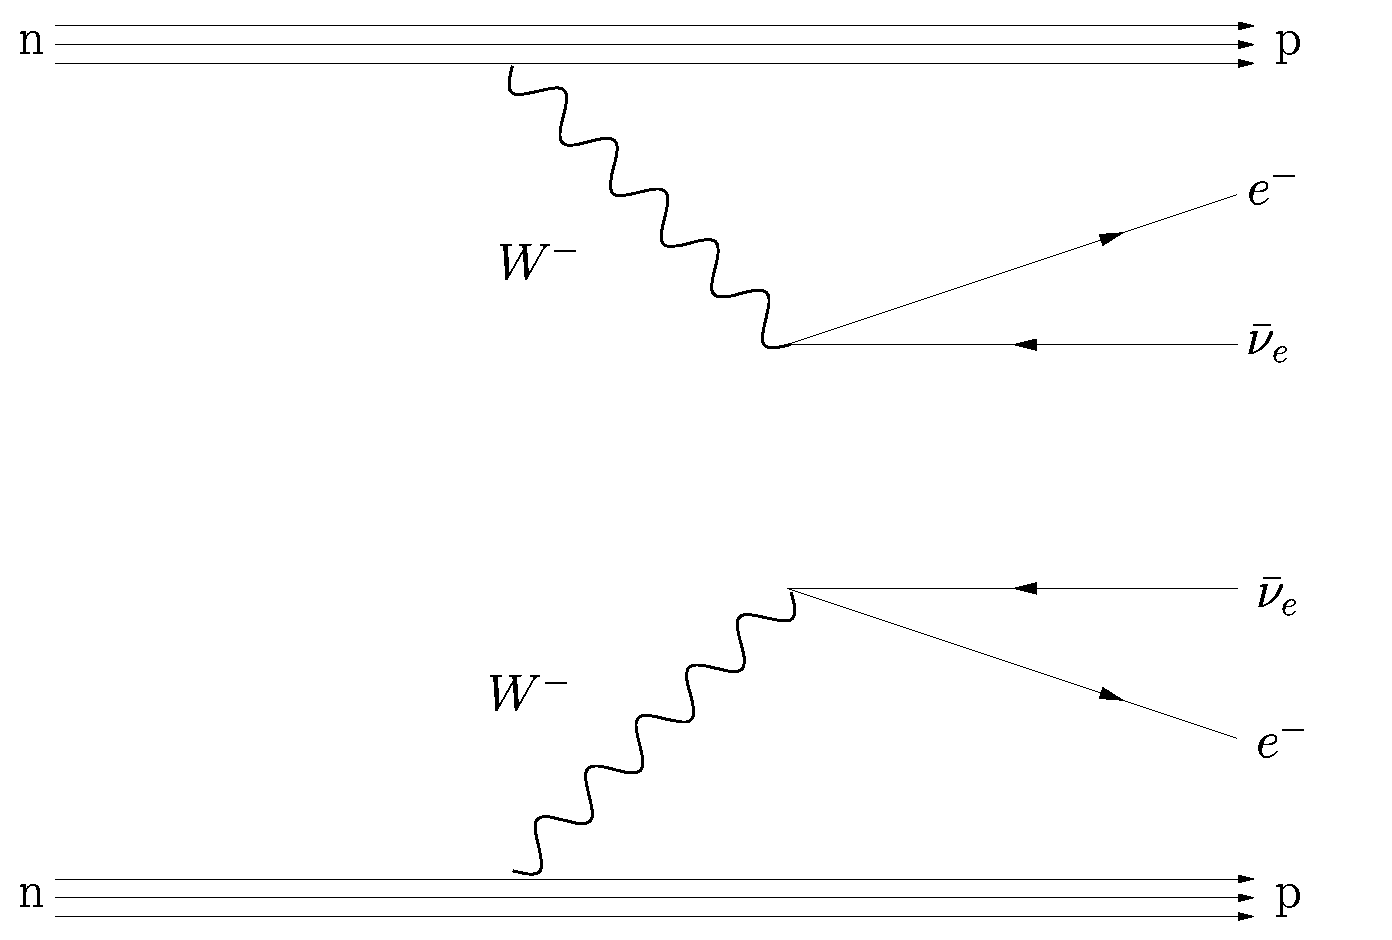
\includegraphics[width=0.4\textwidth]{FD2nu2b.eps} \hfil
  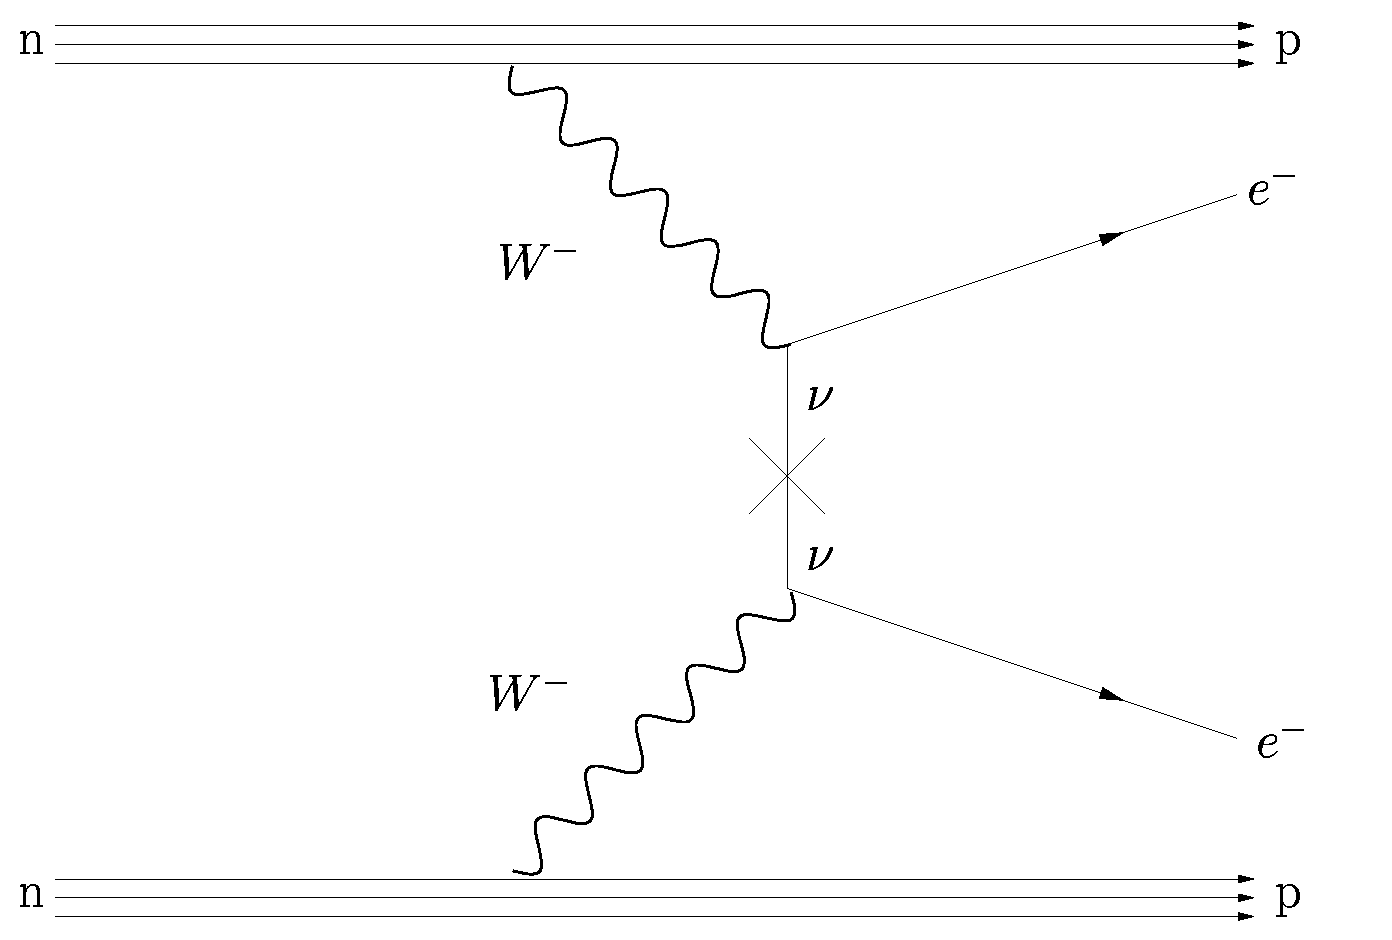
\includegraphics[width=0.4\textwidth]{FD0nu2b.eps}  
  \caption{Feynman diagrams of double beta decay with and without two     neutrinos being emitted.}
  \label{fig:2bdecay}
\end{figure}

According to Fermi's golden rule the rates of these two types of double beta decays are
\begin{equation}
  \label{eq:2nurate}
  1/T^{2\nu}_{1/2} = G_{2\nu}(Q,Z) |\mathcal{M}_{2\nu}|^{2},
\end{equation}
\begin{equation}
  \label{eq:0nurate}
  1/T^{0\nu}_{1/2}=G_{0\nu}(Q,Z)|\mathcal{M}_{0\nu}|^{2}m_{\beta\beta}^{2},
\end{equation}
where the phase space factors $G_{2\nu}(Q,Z)$ and $G_{0\nu}(Q,Z)$ depend on the $Q$-value and the nuclear charge $Z$; the nuclear matrix elements $\mathcal{M}_{2\nu}$ and $\mathcal{M}_{0\nu}$ describe the hadronic part of the decays; and the effective Majorana neutrino mass  $m_{\beta\beta}$ can be expressed as
\begin{equation}
  \label{eq:effmass}
  m_{\beta\beta} \equiv \left| \sum_{k}m_{k}U^{2}_{ek}
  \right| = \left| m_{1}|U_{e1}|^{2} +
    m_{2}|U_{e2}|^{2}e^{i(\alpha_{2}-\alpha_{1})} +
    m_{3}|U_{e3}|^{2}e^{-i(\alpha_{1}+2\delta)} \right|,
\end{equation}
assuming only the exchange of three light neutrinos.

Figure~\ref{fig:m2bVSlightest}, taken from Ref.~\cite{Str05}, shows the expected range of the effective Majorana neutrino mass $m_{\beta\beta}$ as a function of the lightest neutrino mass. The regions marked $\Delta m^{2}_{32}<0$ and $\Delta m^{2}_{32}>0$ are the allowed regions in case of inverted and normal hierarchy, respectively. The effective Majorana neutrino mass $m_{\beta\beta}$ could be invisibly small in case of a normal hierarchy, because the terms in eq.~\ref{eq:effmass} can cancel if the CP-violation phases $\alpha_{1}, \alpha_{2}$ and $\delta$ take special values. An experiment sensitive to $ m_{\beta\beta} \sim 10$~meV would have an excellent chance to see a signal in case of an inverted mass hierarchy. And if the observed $m_{\beta\beta}$ is far below $10$meV, the inverted mass hierarchy can be ruled out. Currently the best constraint $m_{\beta\beta}<0.19 \sim 0.68$ (depending on the choice of nuclear matrix elements) comes from CUORICINO experiment~\cite{Cuo08}. There is also a claim from part of the Heidelberg-Moscow (HdM in short) Collaboration that $m_{\beta\beta} = 0.2 \sim 0.6$~eV (99\% CL)~\cite{Hei04}.
\begin{figure}[tbhp]
  \centering
  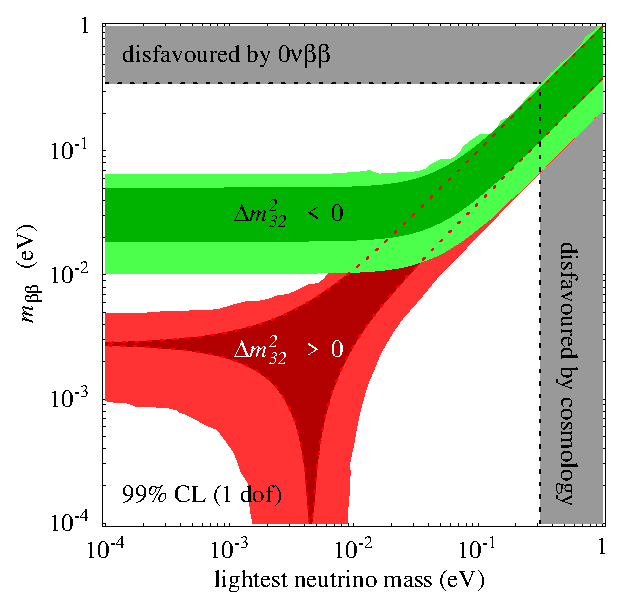
\includegraphics[width=0.5\textwidth]{m2bVSlightest.eps}  
  \caption{Expected range of the effective Majorana neutrino mass     $m_{\beta\beta}$ as function of the lightest neutrino mass (taken     from Ref.~\cite{Str05}). The regions noted with $\Delta     m^{2}_{32}<0$ and $\Delta m^{2}_{32}>0$ are the allowed regions at     99\% confidence level (CL) in case of inverted and normal     hierarchy, respectively. The darker lines in the middle of the     regions correspond to the central values of the oscillation     parameters. And the inner/outer bands correspond to calculations     without/with the $3 \sigma$-uncertainties on the oscillation     parameters.}
  \label{fig:m2bVSlightest}
\end{figure}

\subsection{Combined analysis}
\label{sec:joian}
The constraints on the neutrino mass from cosmological observations, single beta decay and $0\nu\beta\beta$ decay experiments cannot be compared directly because they refer to different observables, $\Sigma, m_{\beta}$ and $m_{\beta\beta}$. However, all being functions of neutrino masses and oscillation parameters, they can be used in a combined analysis. 

Figure~\ref{fig:sum1b2b}, taken from Ref.~\cite{Fog07}, shows regions allowed at $2\sigma$ by neutrino oscillation data, in each of the three coordinate planes of the parameter space ($\Sigma, m_{\beta}$, $m_{\beta\beta}$), for both normal and inverted hierarchy. The most ``aggressive'' cosmological constraint (labeled as 7 in the top left plot of Fig.~\ref{fig:sum1b2b}) already conflicts with the HdM claim on $m_{\beta\beta}$. And the planned sensitivity of KATRIN can confirm or refute the HdM claim.
\begin{figure}[tbhp]
  \centering
  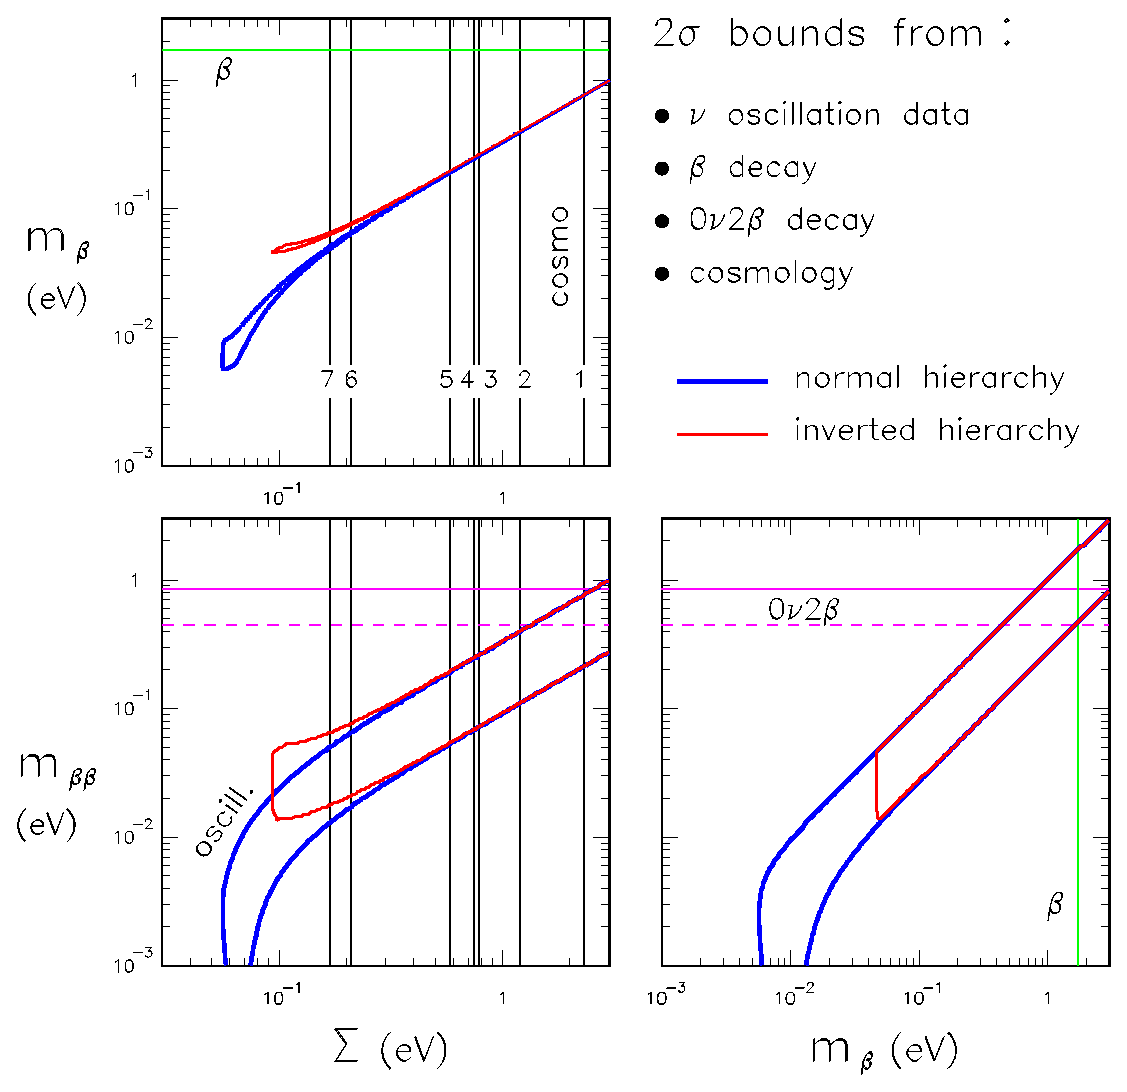
\includegraphics[width=0.8\textwidth]{sum1b2b.eps}  
  \caption{Regions allowed at $2\sigma$ by neutrino oscillation data,     in each of the three coordinate planes of the parameter space     ($\Sigma, m_{\beta}$, $m_{\beta\beta}$), for both normal and     inverted hierarchy (taken from Ref.~\cite{Fog07}). Cosmological     constraints are labeled with numbers corresponding to different     data sets and models from the most conservative one (1) to the     most ``aggressive'' one (7). The plot is taken from     Ref.~\cite{Fog07}.}
  \label{fig:sum1b2b}
\end{figure}

\subsection{Other approaches}
\label{sec:otap}
The effective muon neutrino mass can be obtained from the pion decay $\pi \rightarrow \mu \nu_{\mu}$. Since the masses of the pion $m_{\pi}$ and the muon $m_{\mu}$ are known, the muon neutrino mass can be calculated as $m_{\nu_{\mu}} = m^{2}_{\pi} + m^{2}_{\mu} - 2m_{\pi} (p^{2}_{\mu} + m^{2}_{\mu})^{1/2}$, where $p_{\mu}$ is the muon momentum. The difficulty is to precisely measure $p_{\mu}$. Currently the best limit is $m_{\nu_{\mu}} < 170$ keV (90\% CL)~\cite{Ass96}. New experiments like NuMass aim at a sensitivity of $\sim 8$ keV~\cite{Num20}, which is not competitive with the approaches mentioned before.

It is also possible to measure the absolute neutrino masses by studying neutrino pair emission from meta-stable excited atoms~\cite{Yos07}. The emission rate scales with the fifth power of  the neutrino mass; hence is very small. Novel mechanisms which could largely enhance the rate are needed. The rate also depends on the nature of neutrinos; hence could be used to distinguish between Dirac and Majorana neutrinos.

In the Standard Model extended to include Dirac neutrino masses (see Sec.~\ref{sec:dirac}) the neutrino magnetic moment $\mu_{\nu}$ is proportional to the neutrino mass: $\mu_{\nu} = 3.2 \times 10^{-19}(m_{\nu}/$eV$)\mu_{B}$~\cite{Fuj80}, where $\mu_{B}$ is the Bohr magneton. It is unobservably small given the known upper bounds on neutrino masses. For Majorana neutrinos only transition moments are allowed. The transition moment could convert left-handed neutrinos to right-handed anti-neutrinos of a different flavor. The interaction of the transition moment with the solar magnetic field was used to explain the solar neutrino deficit by Lim and Marciano~\cite{Lim88} and by Akhmedov ~\cite{Akh88} (LMA). The expected magnitude of the transition moment is $\sim 10^{-11}\mu_{B}$. The current best limit, $2 \times 10^{-10}\mu_{B}$, comes from a combined analysis of solar and reactor data~\cite{Gri02}.

%%% Local Variables:
%%% mode:latex
%%% TeX-master: "thesis"
%%% End:
